\documentclass{article}
\usepackage{graphicx}

\usepackage{subfigure}
\usepackage{hyperref}
\usepackage{amsmath}

\usepackage{pifont}% http://ctan.org/pkg/pifont
\newcommand{\cmark}{\ding{51}}%
\newcommand{\xmark}{\ding{55}}%

\begin{document}

\title{Case Study: Total Deterministic (\textit{TD})(Bijection) Consistency Relation}
%\author{Author's Name}

\maketitle

%\begin{abstract}
%The abstract text goes here.
%\end{abstract}

\section{Motivation and origin}

Reversible conversions are very common.
%Suggested by Dr Perdita Stevens \cite{Perdita}.

\section{Specification}
\label{sec:spec}

\subsection{Metamodels (\textit{M,N})}
\label{sec:metamodels}

\begin{figure}[ht]
    \centering
    \mbox{\subfigure[M]{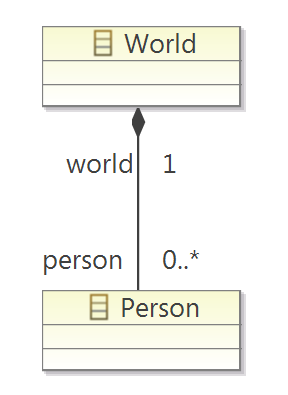
\includegraphics[scale=0.25]{graphics/bij-M.png}}\quad
          \subfigure[N]{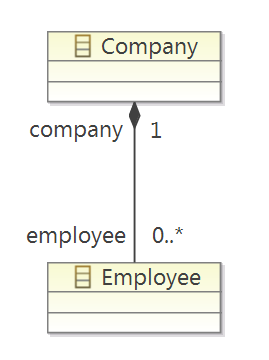
\includegraphics[scale=0.28]{graphics/bij-N.png}}
          }
    \caption{Metamodels}
    \label{fig:Meta}
\end{figure}


\subsection{Consistency relation (\textit{R})}
\label{sec:CR}
~\\
\textbf{Type:} \textit{TD} (Bijection)\\

For every $M$ instance there
exists exactly one $N$ instance such that both are related by $R$ (and vice versa).

~\\

\begin{center}
\begin{tabular}{| c | c | c | c | c | }
  \hline                        
   & injective & entire & simple & surjective \\
  \hline 
  $R$ & \cmark & \cmark & \cmark & \cmark\\
  \hline  
\end{tabular}
\end{center}


\textbf{Definition}\\

For every \textit{Person} in the \textit{World} there
exists exactly one \textit{Employee} in the \textit{Company} (and vice versa)\footnote{Consider there exists only one \textit{World} and one \textit{Company} as containers. Actually they were only defined since \textit{Ecore} forces us to choose an instance root element, and nor \textit{Person} nor \textit{Employee} was an option since we want to model instances with multiple of these elements.}.


%------------------------------------
\pagebreak
\section{Test instances (\textit{m,n})}

\subsection{One person}
\label{sec:one-person}

\begin{figure}[ht]
    \centering
    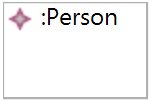
\includegraphics[scale=0.35]{graphics/bij-one-person.png}
    \caption{One person ($m$)}
    \label{fig:I1}
\end{figure}

\subsection{Two employees}
\label{sec:two-employees}

\begin{figure}[ht]
    \centering
    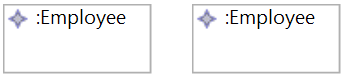
\includegraphics[scale=0.45]{graphics/bij-two-employees.png}
    \caption{Two employees ($n$)}
    \label{fig:I2}
\end{figure}

\subsection{Two persons}
\label{sec:two-persons}

\begin{figure}[ht]
    \centering
    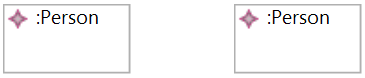
\includegraphics[scale=0.45]{graphics/bij-two-persons.png}
    \caption{Two persons ($m$)}
    \label{fig:I3}
\end{figure}

\subsection{No persons}
\label{sec:no-persons}

\begin{center}
\textit{No persons ($m$)}
\end{center}

\subsection{No employees}
\label{sec:no-employees}

\begin{center}
\textit{No employees ($n$)}
\end{center}

\pagebreak

\subsection{Transformations to assess}
~\\
\begin{center}
\begin{tabular}{| c | c | c | c | c | }
  \hline                        
   & $m$ & $n$ & $\overrightarrow{R}$ & $\overleftarrow{R}$ \\
  \hline 
  T1 & \nameref{sec:one-person} & \nameref{sec:two-employees} & \cmark & \\
  \hline
  T2 & \nameref{sec:one-person} & \nameref{sec:two-employees} & & \cmark \\
  \hline  
  T3 & \nameref{sec:two-persons} & \nameref{sec:two-employees} & \cmark &  \\
  \hline
  T4 & \nameref{sec:one-person} & \nameref{sec:no-employees} & \cmark &  \\
  \hline
  T5 & \nameref{sec:no-persons} & \nameref{sec:no-employees} & \cmark &  \\
  \hline  
\end{tabular}
\end{center}
~\\

%------------------------------------
\pagebreak
\section{Tools assessment}

\subsection{\textit{eMoflon}}

\subsubsection{Specification implementation}

\textit{Specification environment}: Enterprise Architect~\cite{EA}
~\\

\textbf{Metamodels}

\begin{figure}[ht]
    \centering
    \mbox{\subfigure[WorldMM ($M$)]{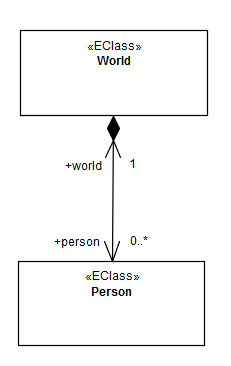
\includegraphics[scale=0.45]{graphics/bij-EA-WorldMM.png}}\quad
          \subfigure[CompanyMM ($N$)]{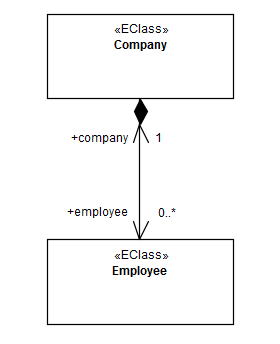
\includegraphics[scale=0.45]{graphics/bij-EA-CompanyMM.png}}
          }
    \caption{Metamodels modelled as EA Ecore Diagrams}
    \label{fig:eMoIMP1}
\end{figure}

~\\
\textbf{Consistency Relation}

\begin{figure}[ht]
  \centering 
  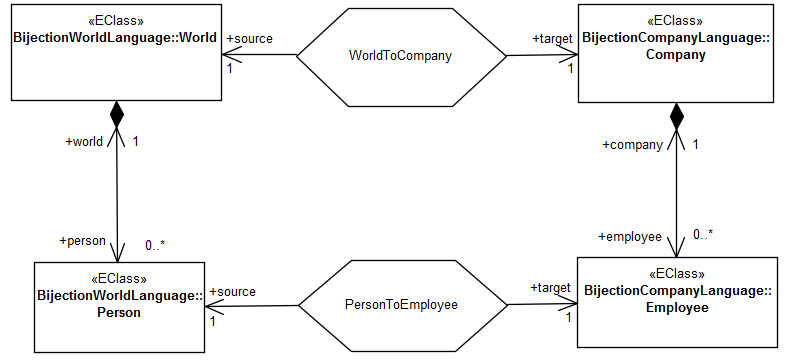
\includegraphics[scale=0.4]{graphics/bij-schema.png}
  \caption{\textit{TGG Schema Diagram}}
  \label{fig:bij-schema}
\end{figure}

\begin{figure}[ht]
  \centering 
  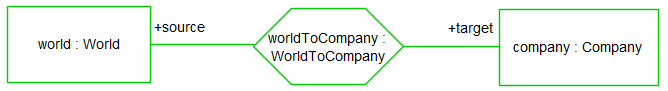
\includegraphics[scale=0.5]{graphics/bij-world-to-company-rule.png}
  \caption{\textit{TGG Rule Diagram}}
  \label{fig:bij-world-to-company-rule}
\end{figure}

~\\

\begin{figure}[ht]
  \centering 
  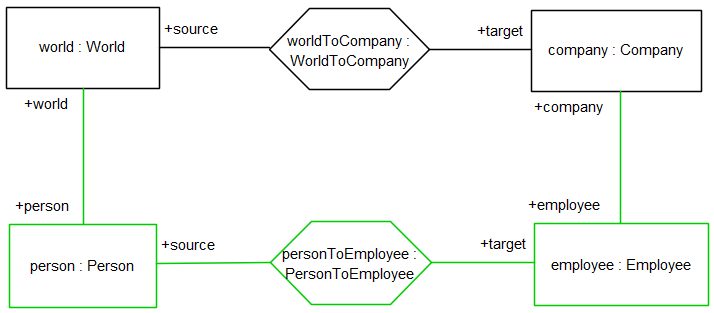
\includegraphics[scale=0.5]{graphics/bij-person-to-employee.png}
  \caption{\textit{TGG Rule Diagram}}
  \label{fig:bij-person-to-employee}
\end{figure}

\subsubsection{Instances transformation results}

\textit{Integration environment}: Eclipse Modelling Tools~\cite{EMT}

~\\

T1 - \nameref{sec:one-person} / \nameref{sec:two-employees} ($\overrightarrow{R}$)
\begin{figure}[ht]
    \centering
    \mbox{\subfigure[$m$]{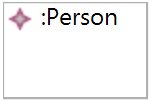
\includegraphics[scale=0.35]{graphics/bij-one-person.png}}\quad\qquad
          \subfigure[$n$]{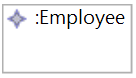
\includegraphics[scale=0.45]{graphics/bij-one-employee.png}}
          }
    \caption{T1 result}
    \label{fig:T1}
\end{figure}

\pagebreak

T2 - \nameref{sec:one-person} / \nameref{sec:two-employees} ($\overleftarrow{R}$)
\begin{figure}[ht]
    \centering
    \mbox{\subfigure[$m$]{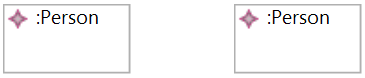
\includegraphics[scale=0.45]{graphics/bij-two-persons.png}}\quad\qquad\quad
          \subfigure[$n$]{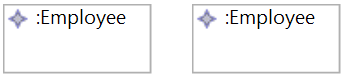
\includegraphics[scale=0.45]{graphics/bij-two-employees.png}}
          }
    \caption{T2 result}
    \label{fig:T2}
\end{figure}

~\\

T3 - \nameref{sec:two-persons} / \nameref{sec:two-employees} ($\overrightarrow{R}$)
\begin{figure}[ht]
    \centering
    \mbox{\subfigure[$m$]{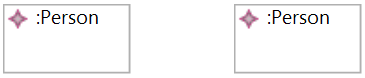
\includegraphics[scale=0.45]{graphics/bij-two-persons.png}}\quad\qquad\quad
          \subfigure[$n$]{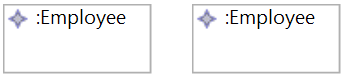
\includegraphics[scale=0.45]{graphics/bij-two-employees.png}}
          }
    \caption{T3 result}
    \label{fig:T3}
\end{figure}

~\\

T4 - \nameref{sec:one-person} / \nameref{sec:no-employees} ($\overrightarrow{R}$)
\begin{figure}[ht]
    \centering
    \mbox{\subfigure[$m$]{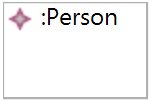
\includegraphics[scale=0.35]{graphics/bij-one-person.png}}\quad\qquad\quad
          \subfigure[$n$]{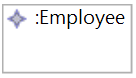
\includegraphics[scale=0.45]{graphics/bij-one-employee.png}}
          }
    \caption{T4 result}
    \label{fig:T4}
\end{figure}

\pagebreak
T5 - \nameref{sec:no-persons} / \nameref{sec:no-employees} ($\overrightarrow{R}$)
\begin{figure}[ht]
    \centering
    \mbox{\subfigure[$m$]{
\includegraphics[scale=0.15]{graphics/bij-empty.png}}\quad\qquad\quad
          \subfigure[$n$]{
\includegraphics[scale=0.15]{graphics/bij-empty.png}}
          }
    \caption{T5 result}
    \label{fig:T5}
\end{figure}

~\\

\subsubsection{Assessment}



\begin{center}
\begin{tabular}{| r | c | }
  \hline                        
  correct & \cmark \\
  \hline
  hippocratic & \cmark \\
  \hline 
  undoable & \cmark \\
  \hline 
  history-ignorant & \cmark \\
  \hline 
  simply-matching & \cmark \\
  \hline 
  matching & \cmark \\
  \hline 
  least-change & \cmark \\
  \hline   
\end{tabular}
\end{center}


%------------------------------------
\pagebreak
\subsection{\textit{Echo}}
\subsubsection{Specification implementation}
\textit{Specification environment}:
~\\

\textbf{Metamodels}
~\\

\textbf{Consistency Relation}


\subsubsection{Instances transformation results}
\textit{Integration environment}:
~\\

T1 - \nameref{sec:one-person} / \nameref{sec:two-employees} ($\overrightarrow{R}$)

~\\

T2 - \nameref{sec:one-person} / \nameref{sec:two-employees} ($\overleftarrow{R}$)

~\\

T3 - \nameref{sec:two-persons} / \nameref{sec:two-employees} ($\overrightarrow{R}$)

~\\

T4 - \nameref{sec:one-person} / \nameref{sec:no-employees} ($\overrightarrow{R}$)

~\\

T5 - \nameref{sec:no-persons} / \nameref{sec:no-employees} ($\overrightarrow{R}$)

\subsubsection{Assessment}

\begin{center}
\begin{tabular}{| r | c |}
  \hline                        
  correct & \\
  \hline
  hippocratic & \\
  \hline 
  undoable & \\
  \hline 
  history-ignorant & \\
  \hline 
  simply-matching & \\
  \hline 
  matching & \\
  \hline 
  least-change & \\
  \hline   
\end{tabular}
\end{center}

%------------------------------------
\pagebreak
\subsection{\textit{Focal}}
\subsubsection{Specification implementation}
\textit{Specification environment}:
~\\

\textbf{Metamodels}
~\\

\textbf{Consistency Relation}
\subsubsection{Instances transformation results}
\textit{Integration environment}:
~\\

T1 - \nameref{sec:one-person} / \nameref{sec:two-employees} ($\overrightarrow{R}$)

~\\

T2 - \nameref{sec:one-person} / \nameref{sec:two-employees} ($\overleftarrow{R}$)

~\\

T3 - \nameref{sec:two-persons} / \nameref{sec:two-employees} ($\overrightarrow{R}$)

~\\

T4 - \nameref{sec:one-person} / \nameref{sec:no-employees} ($\overrightarrow{R}$)

~\\

T5 - \nameref{sec:no-persons} / \nameref{sec:no-employees} ($\overrightarrow{R}$)

\subsubsection{Assessment}

\begin{center}
\begin{tabular}{| r | c |}
  \hline                        
  correct & \\
  \hline
  hippocratic & \\
  \hline 
  undoable & \\
  \hline 
  history-ignorant & \\
  \hline 
  simply-matching & \\
  \hline 
  matching & \\
  \hline 
  least-change & \\
  \hline   
\end{tabular}
\end{center}
%-------------------------------------
\pagebreak
\subsection{Summary table and comparison}

\pagebreak
\section{Discussion}

\pagebreak
\begin{thebibliography}{1}

\bibitem{Perdita}http://homepages.inf.ed.ac.uk/perdita/ 

\bibitem{Perdita2}Stevens, Perdita. "Bidirectional model transformations in QVT: Semantic issues and open questions." Model Driven Engineering Languages and Systems. Springer Berlin Heidelberg, 2007. 1-15.

\bibitem{Perdita3}Stevens, Perdita. "Observations relating to the equivalences induced on model sets by bidirectional transformations." Electronic Communications of the EASST 49 (2012).

%------------------

\bibitem{EA}http://www.sparxsystems.com/products/ea/index.html

\bibitem{EMT}http://www.eclipse.org/


\end{thebibliography}



\end{document}